\documentclass{article}

\usepackage{geometry}
\geometry{a4paper}
\setlength{\parindent}{10mm}
\setlength{\parskip}{0.9em}
\def\baselinestretch{1.5}

\usepackage[spanish,mexico]{babel}
%\renewcommand {\spanishtablename}{Tabla}
\usepackage[spanish,onelanguage,ruled]{algorithm2e}
\usepackage[utf8]{inputenc}
\usepackage{graphicx}
\usepackage{caption} 
\usepackage{amsmath, amsthm, amsfonts}
\usepackage{enumerate} 
\usepackage{fancyhdr}
\usepackage{anysize} 
\usepackage[usenames]{color}
\usepackage{booktabs}
\usepackage{etoolbox}
 \usepackage{fancyvrb}
 \usepackage{color,soul}
 \usepackage[dvipsnames]{xcolor}
 \usepackage{graphicx}
\usepackage{subcaption}
\usepackage{listings}
\usepackage{amssymb}

\usepackage{verbatim}
% redefine \VerbatimInput
\RecustomVerbatimCommand{\VerbatimInput}{VerbatimInput}%
 {fontsize=\footnotesize,
  %
  frame=lines,  % top and bottom rule only
  framesep=1em, % separation between frame and text
  rulecolor=\color{Gray},
  %
  label=\fbox{\color{Black}test.txt},
  labelposition=topline,
  %
  %commandchars=\|\(\), % escape character and argument delimiters for
                  % commands within the verbatim
  %commentchar=*        % comment character
 }


\pagestyle{fancy}

\chead{}
\lhead{} 
\rhead{}
\lfoot{\it }
\cfoot{}
\rfoot{\thepage}

\title{
\centering
Modelos Probabilistas Aplicados \\
Johanna Bolaños Zúñiga \\
Matricula: 1883900\\
Tarea 7
}

\date{}

\begin{document}
\maketitle

\section{Introducción}
En el presente trabajo se analizan datos generados con diferentes funciones para mostrar la aplicación de la regresión lineal y el uso de las transformaciones. Este análisis es complementado con resultados obtenidos de experimentos computacionales realizados en el software R versión 4.0.2 \cite{r}. El código empleado se encuentra en el repositorio GitHub \cite{github}.

\section{Regresión lineal}
El análisis de regresión se centra en la exploración, explicación y estudio de dependencia de una variable mediante una o más variables explicativas. El término regresión significa que utilizaremos información pasada y es lineal porqué está bajo el supuesto de que entre dos variables ($x$ y $y$) existe una relación lineal. Cuando se utiliza sólo una variable independiente para tratar de explicar la variable dependiente, es una regresión lineal simple, pero cuando se utilizan más de dos variables independientes o dependientes, se conoce como regresión múltiple.
 

La regresión lineal consiste en generar un modelo de regresión (ecuación de una recta) que permita explicar la relación lineal que existe entre dos variables. A la variable dependientes o respuesta se le identifican como $y$, y a la variables predictoras o independientes como $x$. Las ecuaciones \ref{lineal} y \ref{multiple}, son las ecuaciones estimadas de regresión lineal simple y múltiple, respectivamente,
\begin{equation}
y= b_{1}x + b_{0} + \epsilon , \\ \label{lineal}
\end{equation}
\begin{equation}
y= b_{0} + b_{1}x_{1} + b_{2}x_{2} + \dots + b_{p}x_{p} + \epsilon , \label{multiple}
\end{equation}
\noindent donde $b_{0}$ es la ordenada al origen (el valor de $y$ cuando $x$ es igual a cero) y, $b_{1}$ es la pendiente de la recta (el cambio en $y$ cuando $x$ aumenta en una unidad y $\epsilon$ es el error aleatorio. Este último representa la diferencia entre el valor ajustado por la recta y el valor real. Recoge el efecto de todas aquellas variables que influyen en $y$ pero que no se incluyen en el modelo como predictores. Al error aleatorio también se le conoce como residuo. Los errores, se consideran variables aleatorias independientes distribuidas normalmente con media cero y desviación estándar $\sigma$. Esto implica que el valor
medio o valor esperado de $\hat{y}$ son los mostrados en las ecuaciones \ref{linealest} y \ref{multipleest}, las cuales son las ecuaciones estimadas de regresión lineal simple y múltiple, respectivamente,
\begin{equation}
\hat{y}= \hat{b}_{1}x + \hat{b}_{0} + \epsilon , \\ \label{linealest}
\end{equation}
\begin{equation}
\hat{y}= \hat{b}_{1} + \hat{b}_{1}x_{1} + \hat{b}_{2}x_{2} + \dots + \hat{b}_{p}x_{p} + \epsilon ,
\label{multipleest}
\end{equation}
\noindent donde $\hat{y}$ es el valor estimado (aproximado) de $y$, $\hat{b}_{0}$ y $\hat{b}_{p}$ son estimaciones que se conocen como coeficientes de regresión, ya que toman aquellos valores que minimizan la suma de cuadrados residuales, dando lugar a la recta que pasa más cerca de todos los puntos.

En conclusión, el análisis de regresión consiste en definir la variable independiente $x$ que ayude a explicar (estimar) la variable dependiente $y$, siempre que exista una relación lineal entre ellas, además, de que ambas variables deben ser cuantitativas \cite{gutierrez}.

Para determinar si hay relación lineal entre las variables dependientes e independientes, por lo general, se utilizan las gráficas de dispersión, ya que son ayudas visuales que permiten observar, rápidamente, si existe esta relación. Sin embargo, un análisis más fuerte es determinar la correlación entre los datos, ya que es una medida de la presencia de una relación lineal en datos bivariados (entre dos variables). Hay diferentes definiciones, sin embargo, la comúnmente utilizada, es la de correlación de Pearson (se puede hallar con la función \texttt{cor(x, y)}). Se denota con la letra $r$ y sus valores se interpretan de la siguiente manera:

\begin{itemize}
    \item Cerca de uno: cuando $x$ crece, $y$ crece de manera linealmente dependiente.
    \item Cerca de menos uno: cuando $x$ crece, $y$ disminuye de manera linealmente dependiente (o vice versa).
    \item Cerca de cero: no está presente ninguna relación lineal entre $x$ y $y$.
\end{itemize}

El valor de la correlación se puede hallar con la función \texttt{cor(x, y)} en el programa R. De igual manera, la función \texttt{lm(y$\thicksim$x)}, donde $y$, es la variable dependiente (la que se trata de predecir) y $x$ es la variable predictora (independiente), permite obtener el modelo estimado de regresión lineal de los datos a analizar. Con la función de \texttt{summary} se generan los resultados de este modelo.

Para entender el funcionamiento de la función \texttt{lm} se realizó una serie de experimentos, en los cuales consideramos crear diversas funciones, tanto lineales como no lineales, para la obtención de datos dependientes (variables \texttt{y}).

Para el ejemplo de la regresión lineal simple, se generaron $1,000$ datos a partir de la ecuación $y=8x_{1}+5$, donde $x_{1}$ es un número pseudoaleatorio entre $10$ y $60$. Los resultados obtenidos fueron guardados en un dataframe. Se realizó un diagrama de dispersión (ver figura \ref{ec1} para apreciar la relación entre las variables $x_{1}$ y $y$, en la cual se observa, claramente, la relación lineal entre estas variables.


\begin{figure}
\centering
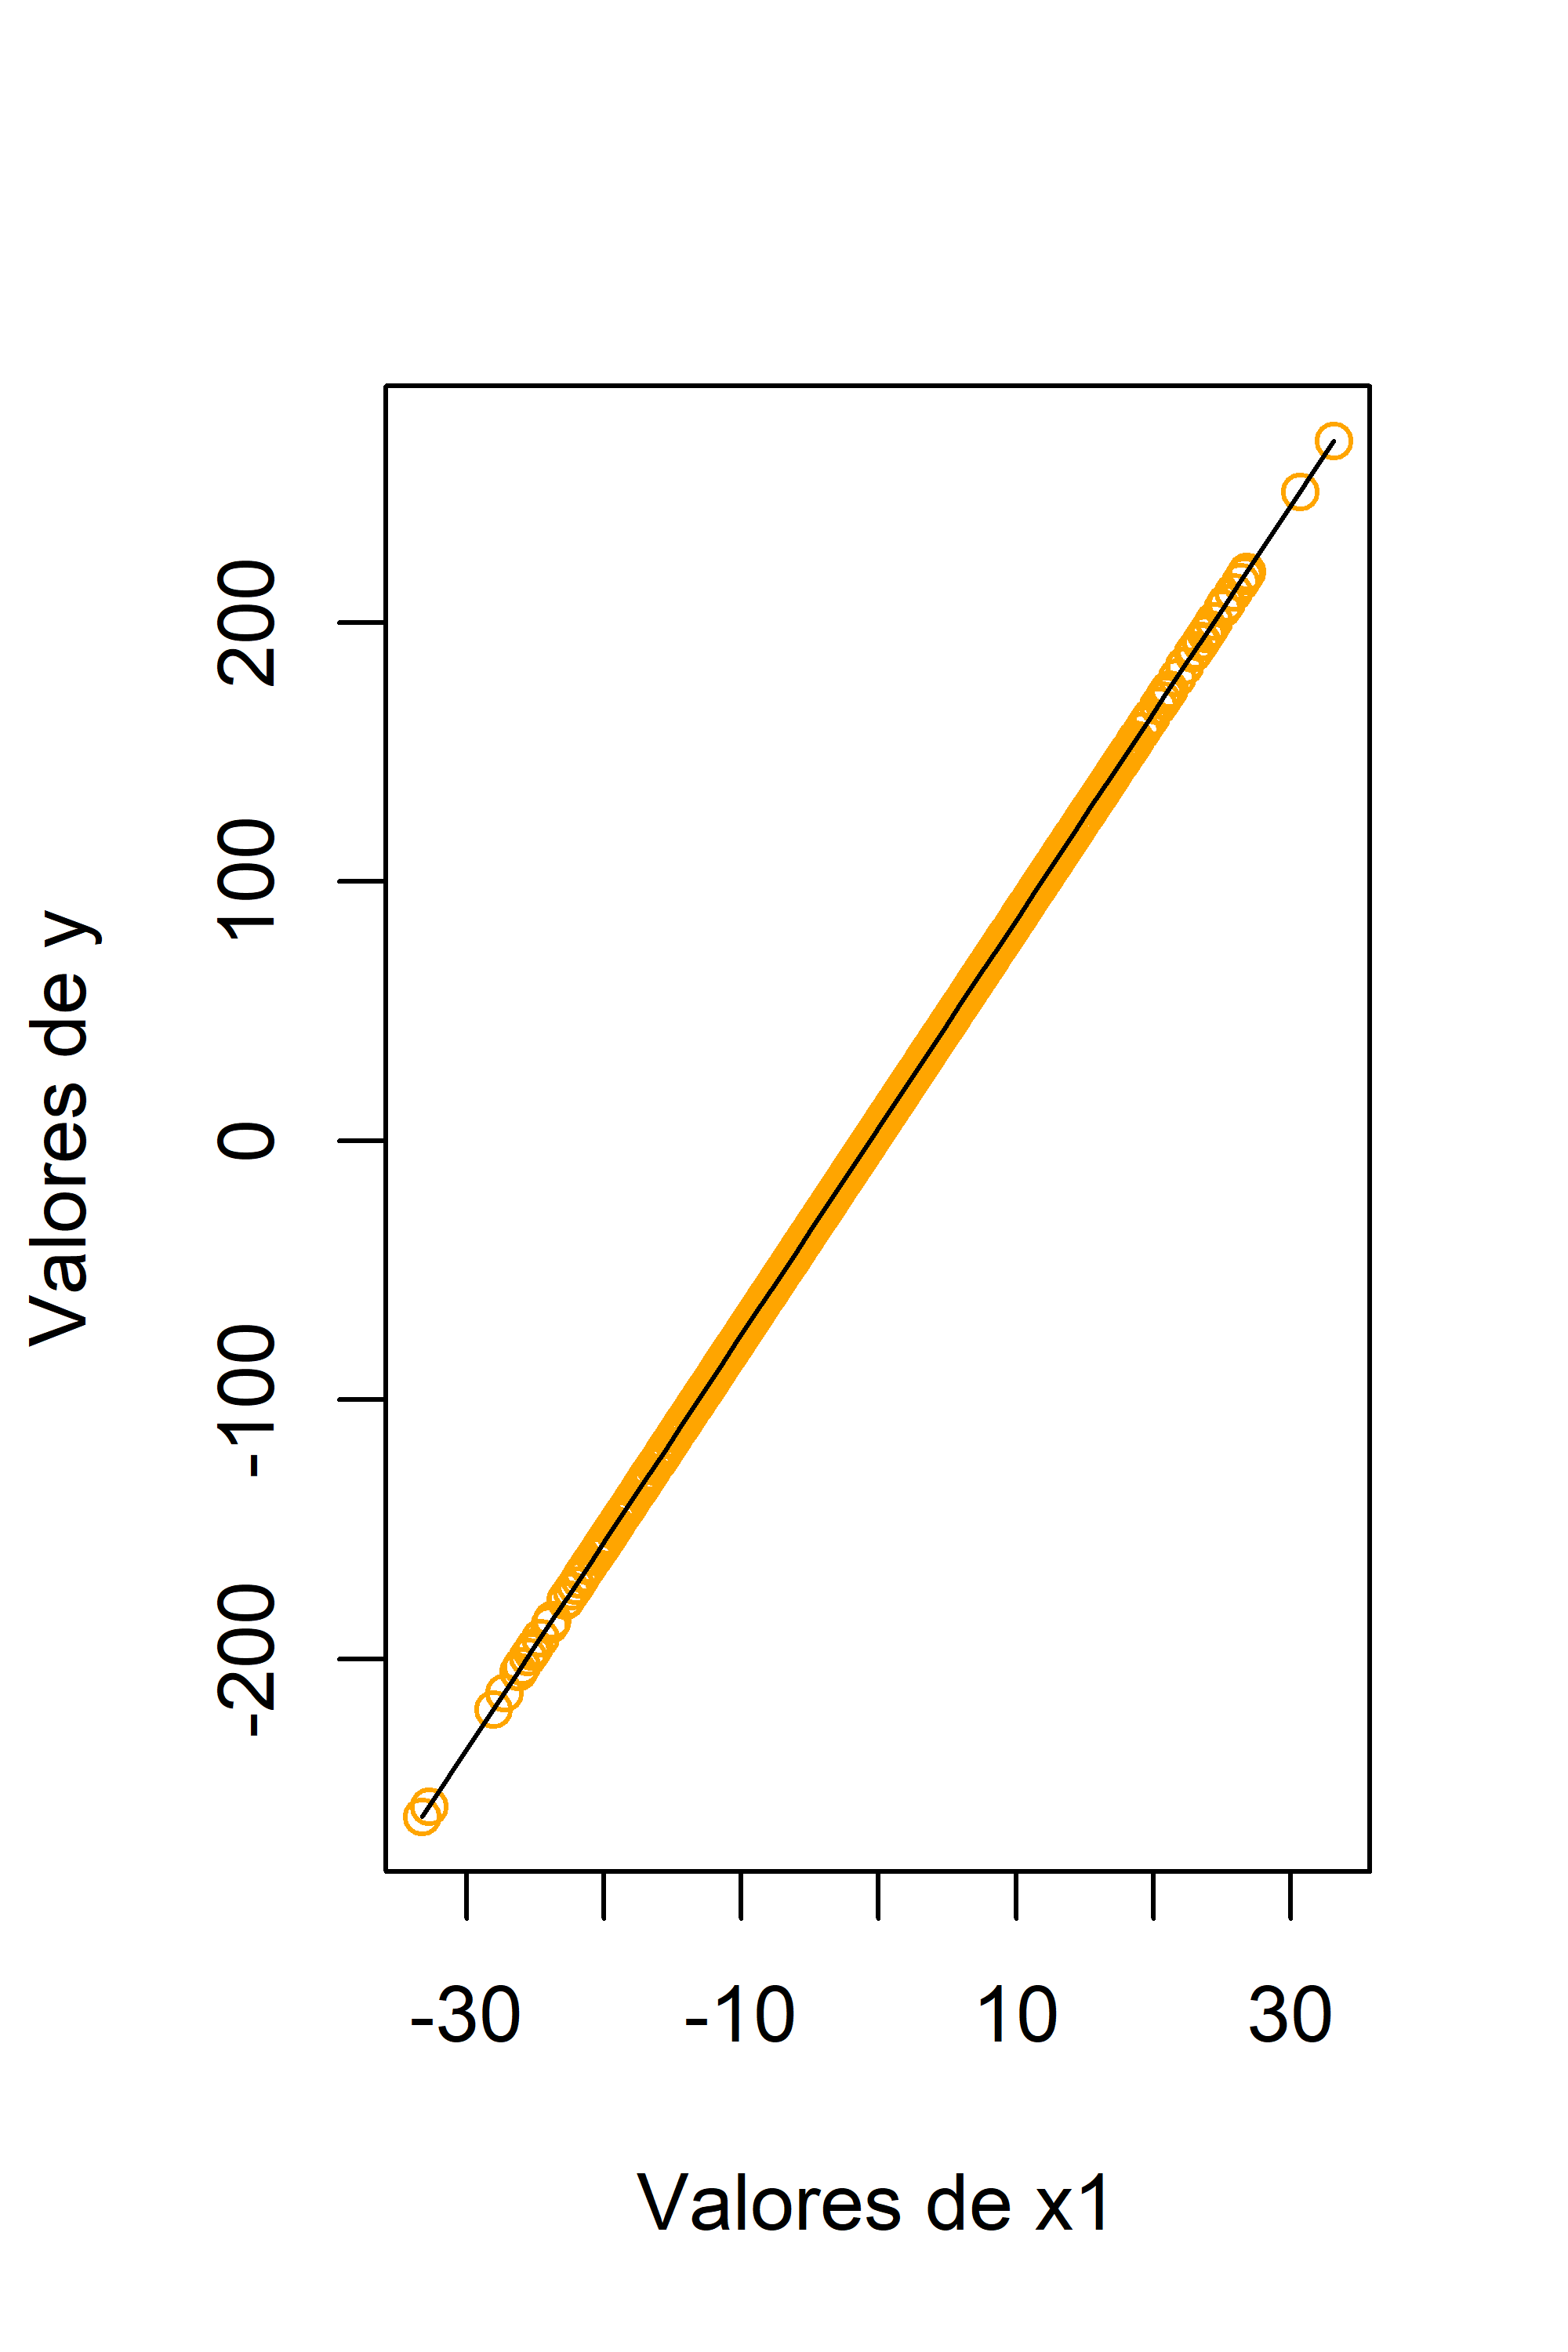
\includegraphics[scale=0.9]{Figures/linealsencilla.png}
\caption{Diagrama de dispersión de los datos provenientes de la ecuación lineal}
\label{ec1}
\end{figure}

\VerbatimInput{Resulpruebas/linealsencilla.txt}

De acuerdo al resultado obtenido de la aplicación de la función \texttt{lm}, se observa que los coeficientes de regresión $\hat{b}_{1} = 8$ y $\hat{b}_{0} = 5$ y $r = 1$, es decir, cuando $x_{1} = 0$, es valor estimado de $y = 8$ y por cada unidad que aumente $x_{1}$ el valor estimado de $y$ aumenta en $8$ unidades. Por lo tanto, el modelo estimado de regresión lineal para estos datos estaría dada como $\hat{y}=8x_{1}+5$ (el cual con anterioridad se tenía). También se realizó el mismo procedimiento considerando que los valores de la variable $x_{1}$ tuvieran una distribución exponencial, normal o uniforme, y se obtuvieron los mismos resultados.

Para la regresión lineal múltiple, también se generaron $1,000$ datos a partir de la ecuación $y=20*x_{1}+5*x_{2}+1$, donde las variable $x_{1}$y $x_{2}$ son pseudoaleatorias uniformes. Los resultados obtenidos fueron guardados en un dataframe. Se utilizo la función \texttt{cor} para determinar la correlación entre estas variables. Las respectivas correlaciones se encuentran graficadas en la figura \ref{multiple}, en la cual se puede observar la dependencia lineal de la varible $y$ con las variables $x_{1}$ y $x_{2}$

\begin{figure}[h]
\centering
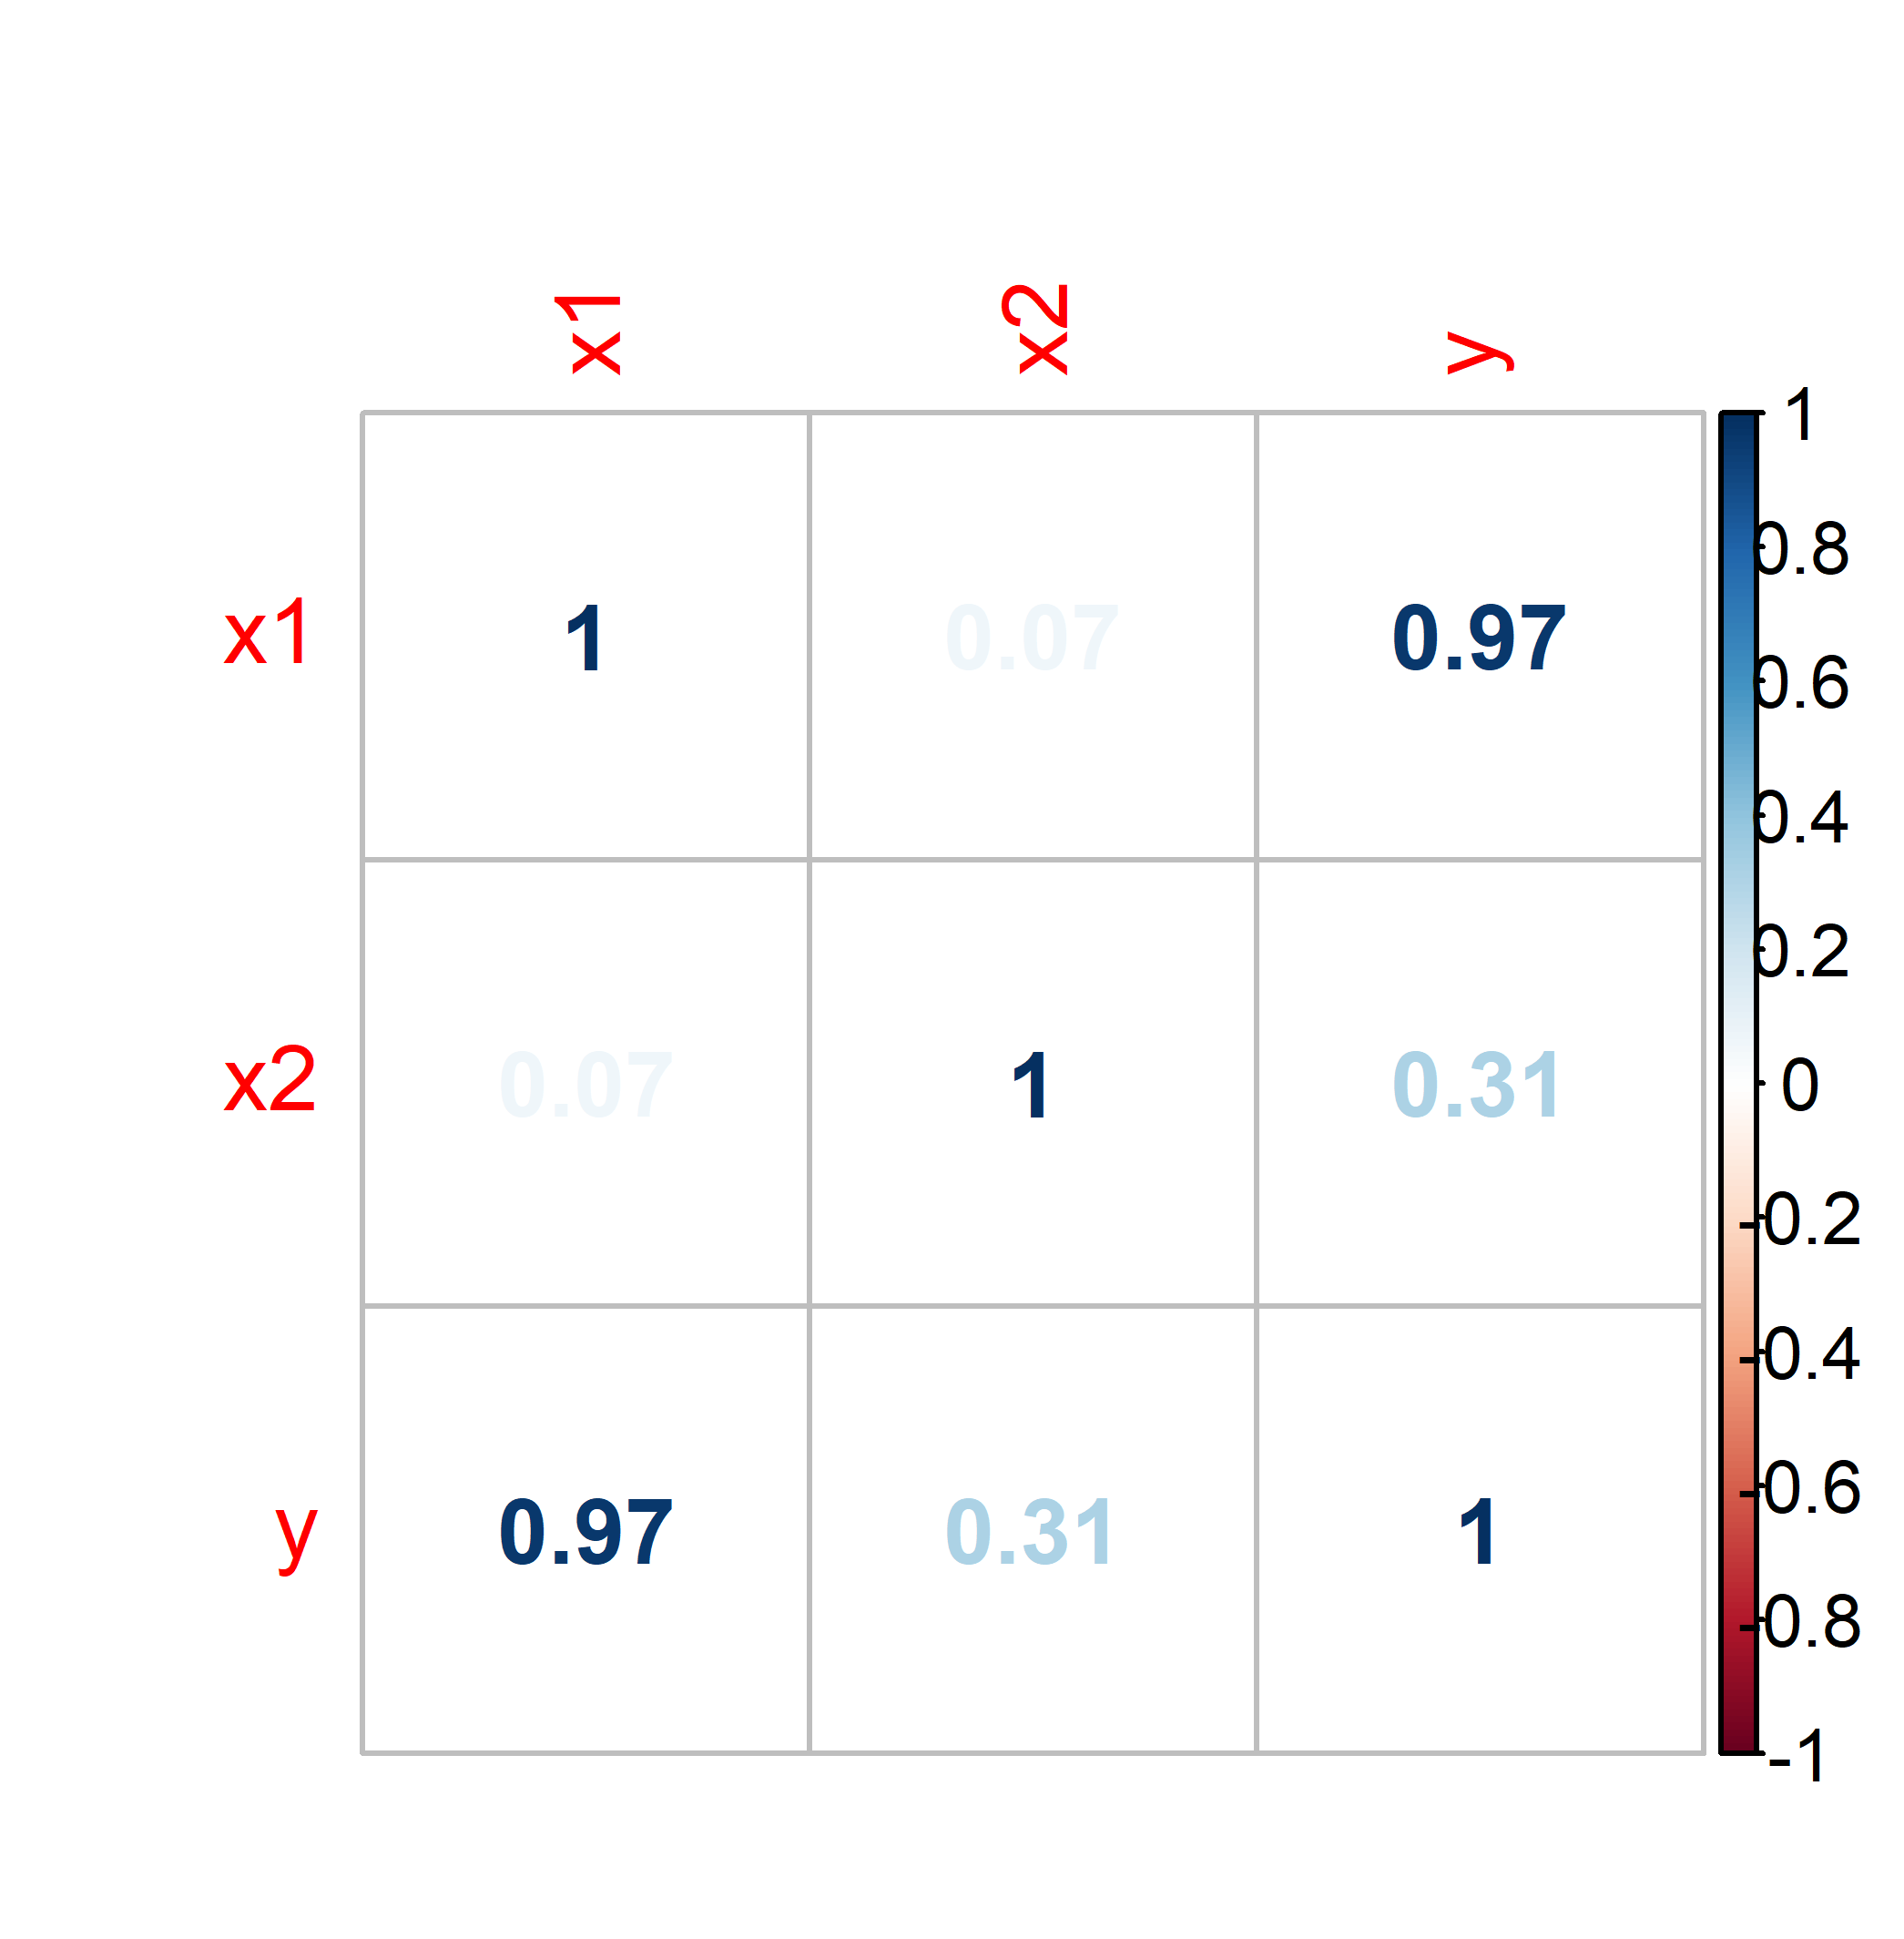
\includegraphics[scale=0.1]{Figures/linealmultiple.png}
\caption{Correlación entre los datos provenientes de una ecuación lineal con dos variables independientes}
\label{ec1}
\end{figure}

\VerbatimInput{Resulpruebas/linealmultiple.txt}

De acuerdo al resultado obtenido de la aplicación de la función \texttt{lm}, se observa que $\hat{b}_{1} = 20$, $\hat{b}_{2} = 5$,  $\hat{b}_{0} = 1$ y $r = 1$. Por lo tanto, el modelo estimado de regresión lineal múltiple para estos datos estaría dada como $\hat{y}=20x_{1}+5x_{2}+1$. También se realizó el mismo procedimiento considerando que los valores de las variables $x_{1}$ y  $x_{2}$ tuvieran una distribución exponencial, normal o sin una distribución específica y se obtuvieron los mismos resultados.

Hasta aquí, se ha realizado el análisis con datos de los cuales se conocía su comportamiento, sin embargo, en los casos reales, este comportamiento no se conoce y no siempre es lineal, lo cual aumenta la complejidad del análisis de estos y la predicción de su comportamiento, haciendo necesario ajustar la tendencia de los datos a un modelo lineal ya que esto facilita el análisis y la predicción de su comportamiento para la toma de decisiones. Para llevar a cabo este ajuste se utilizan las transformaciones.

\section{Transformaciones}
La meta de las transformaciones es acomodar los datos a una relación lineal, ya que bajo este criterio se facilita el análisis y la predicción del comportamiento de estos.

De acuerdo a Mangiafico \cite{mangiafico}, para datos sesgados a la derecha o izquierda (sesgo positivo y negativo, respectivamente), las transformaciones comunes incluyen raíz cuadrada, raíz cúbica y logaritmo. Otro enfoque es utilizar la transformación de Box-Cox, la cual determina un valor lambda ($\lambda$), que se utiliza como coeficiente de potencia para transformar los valores. El procedimiento Box\textendash Cox se realiza mediante la función \texttt{boxcox} en el programa R. Esta utiliza un procedimiento de \textit{log-likelihood} para encontrar la lambda que se utilizará para transformar la variable dependiente de un modelo lineal (una regresión lineal). Cabe mencionar que estas transformaciones solo se pueden aplicar sobre variables de respuesta (variables dependientes) estrictamente positivas.

En este trabajo se utilizó las transformaciones logarítmicas, raíz cuadrada y Box\textendash Cox. Para determinar que tipo de transformación es la más apropiada, se utilizó el coeficiente de determinación ($R^2$), el cual es una medida de la bondad de ajuste de la recta estimada a los datos reales, es decir, entre más cercano esté este valor a la unidad, la transformación tendrá un mejor ajuste. Este coeficiente se calcula elevando al cuadrado el valor de \textit{r} en los modelos de regresión lineal simple el valor de ($R^2$), sin embargo, no es así en regresión múltiple. Existe una modificación de ($R^2$) conocida como ($R^2-ajustado$) que se emplea principalmente en los modelos de regresión múltiple, el cual introduce una penalización cuantos más predictores se incorporan al modelo.

Para el análisis de las trasformaciones, se generaron $1,000$ datos a partir de la ecuación cuadrática de la forma $y=3x_{1}1^2 + rnorm(n)$, donde $x_{1}$ es un número pseudoaleatorio entre $10$ y $60$ y $n$ son las réplicas. Los resultados obtenidos fueron guardados en un dataframe. Se realizó un diagrama de dispersión (ver figura \ref{f3} para apreciar la relación entre las variables $x_{1}$ y $y$), en la cual se observa, claramente, que hay una relación entre estas variables, pero no es lineal, por lo que se procedió a realizar tres diferentes transformaciones.

\begin{figure}
\centering
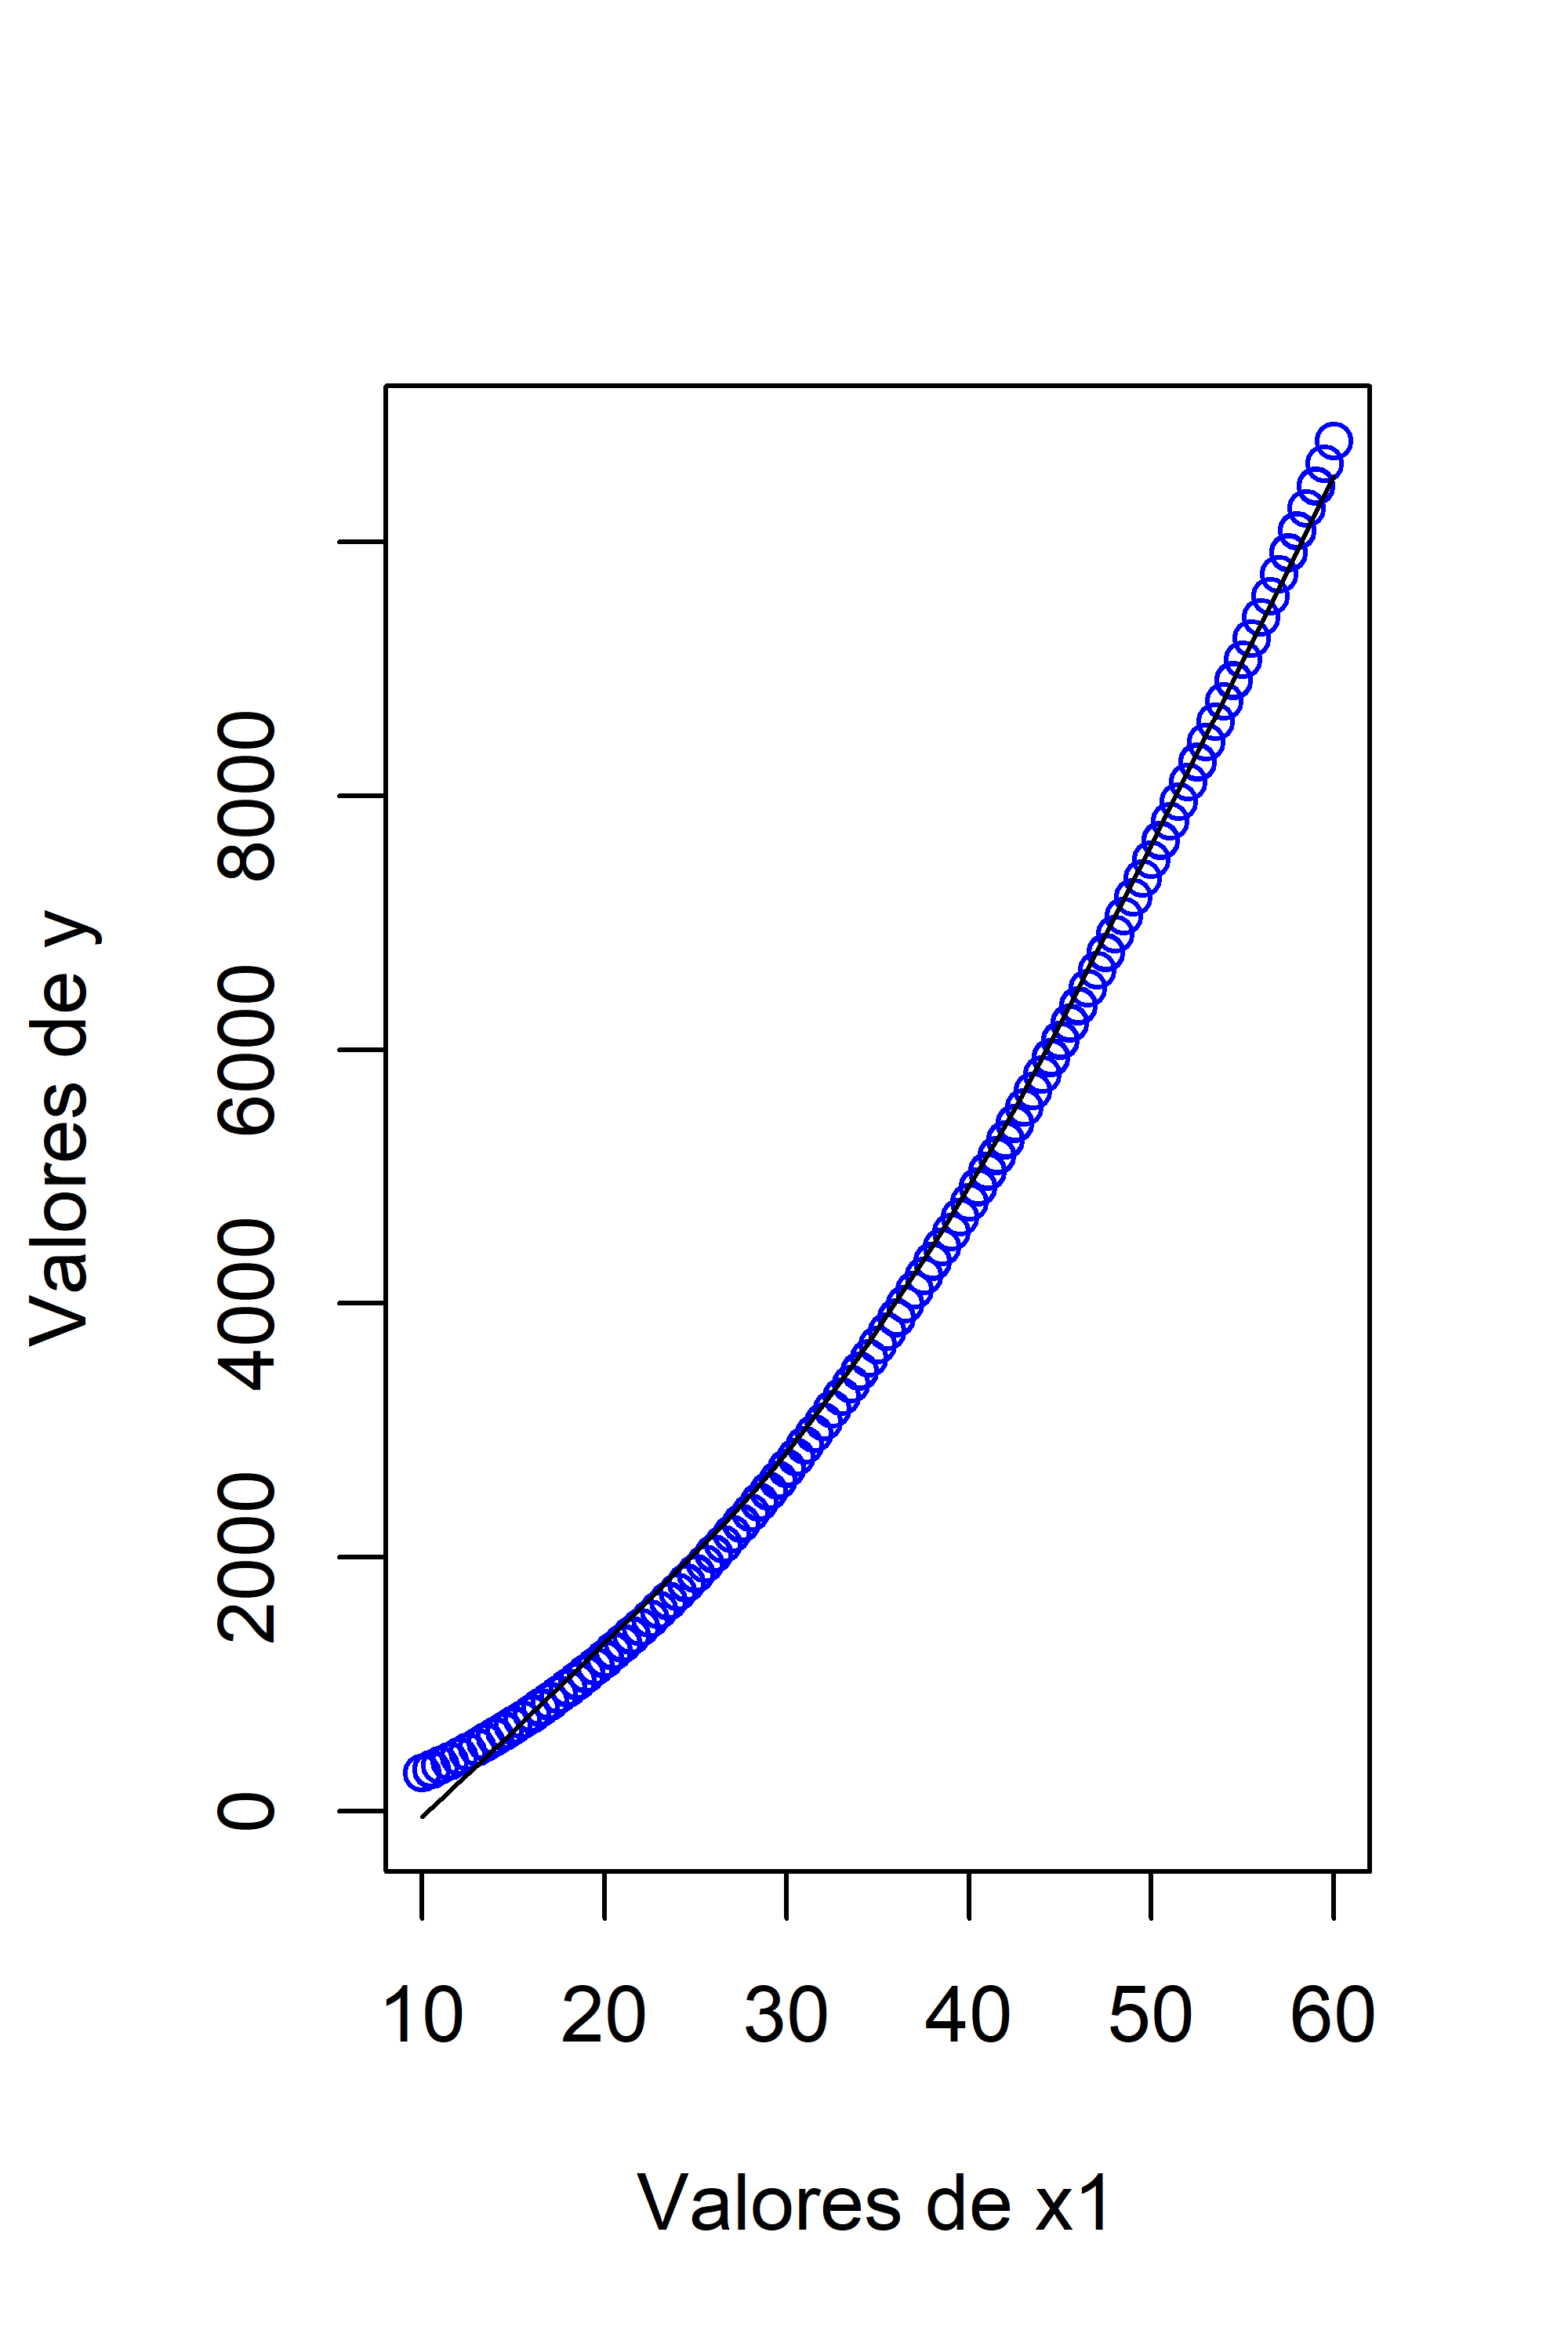
\includegraphics[scale=0.9]{Figures/cuadratica.png}
\caption{Diagrama de dispersión de los datos generados a partir de una función cuadrática}
\label{f3}
\end{figure}

En la figura \ref{tlog}, se muestra el comparativo de los diagramas de dispersión de las transformaciones logarítmicas aplicadas, tanto a los datos de las variables $x$, como a $y$ y a ambas, en la cual podemos observar que se obtiene un ajuste lineal a los datos cuando se aplica la transformación logarítmica a $x$ y $y$.

\begin{figure}
\centering
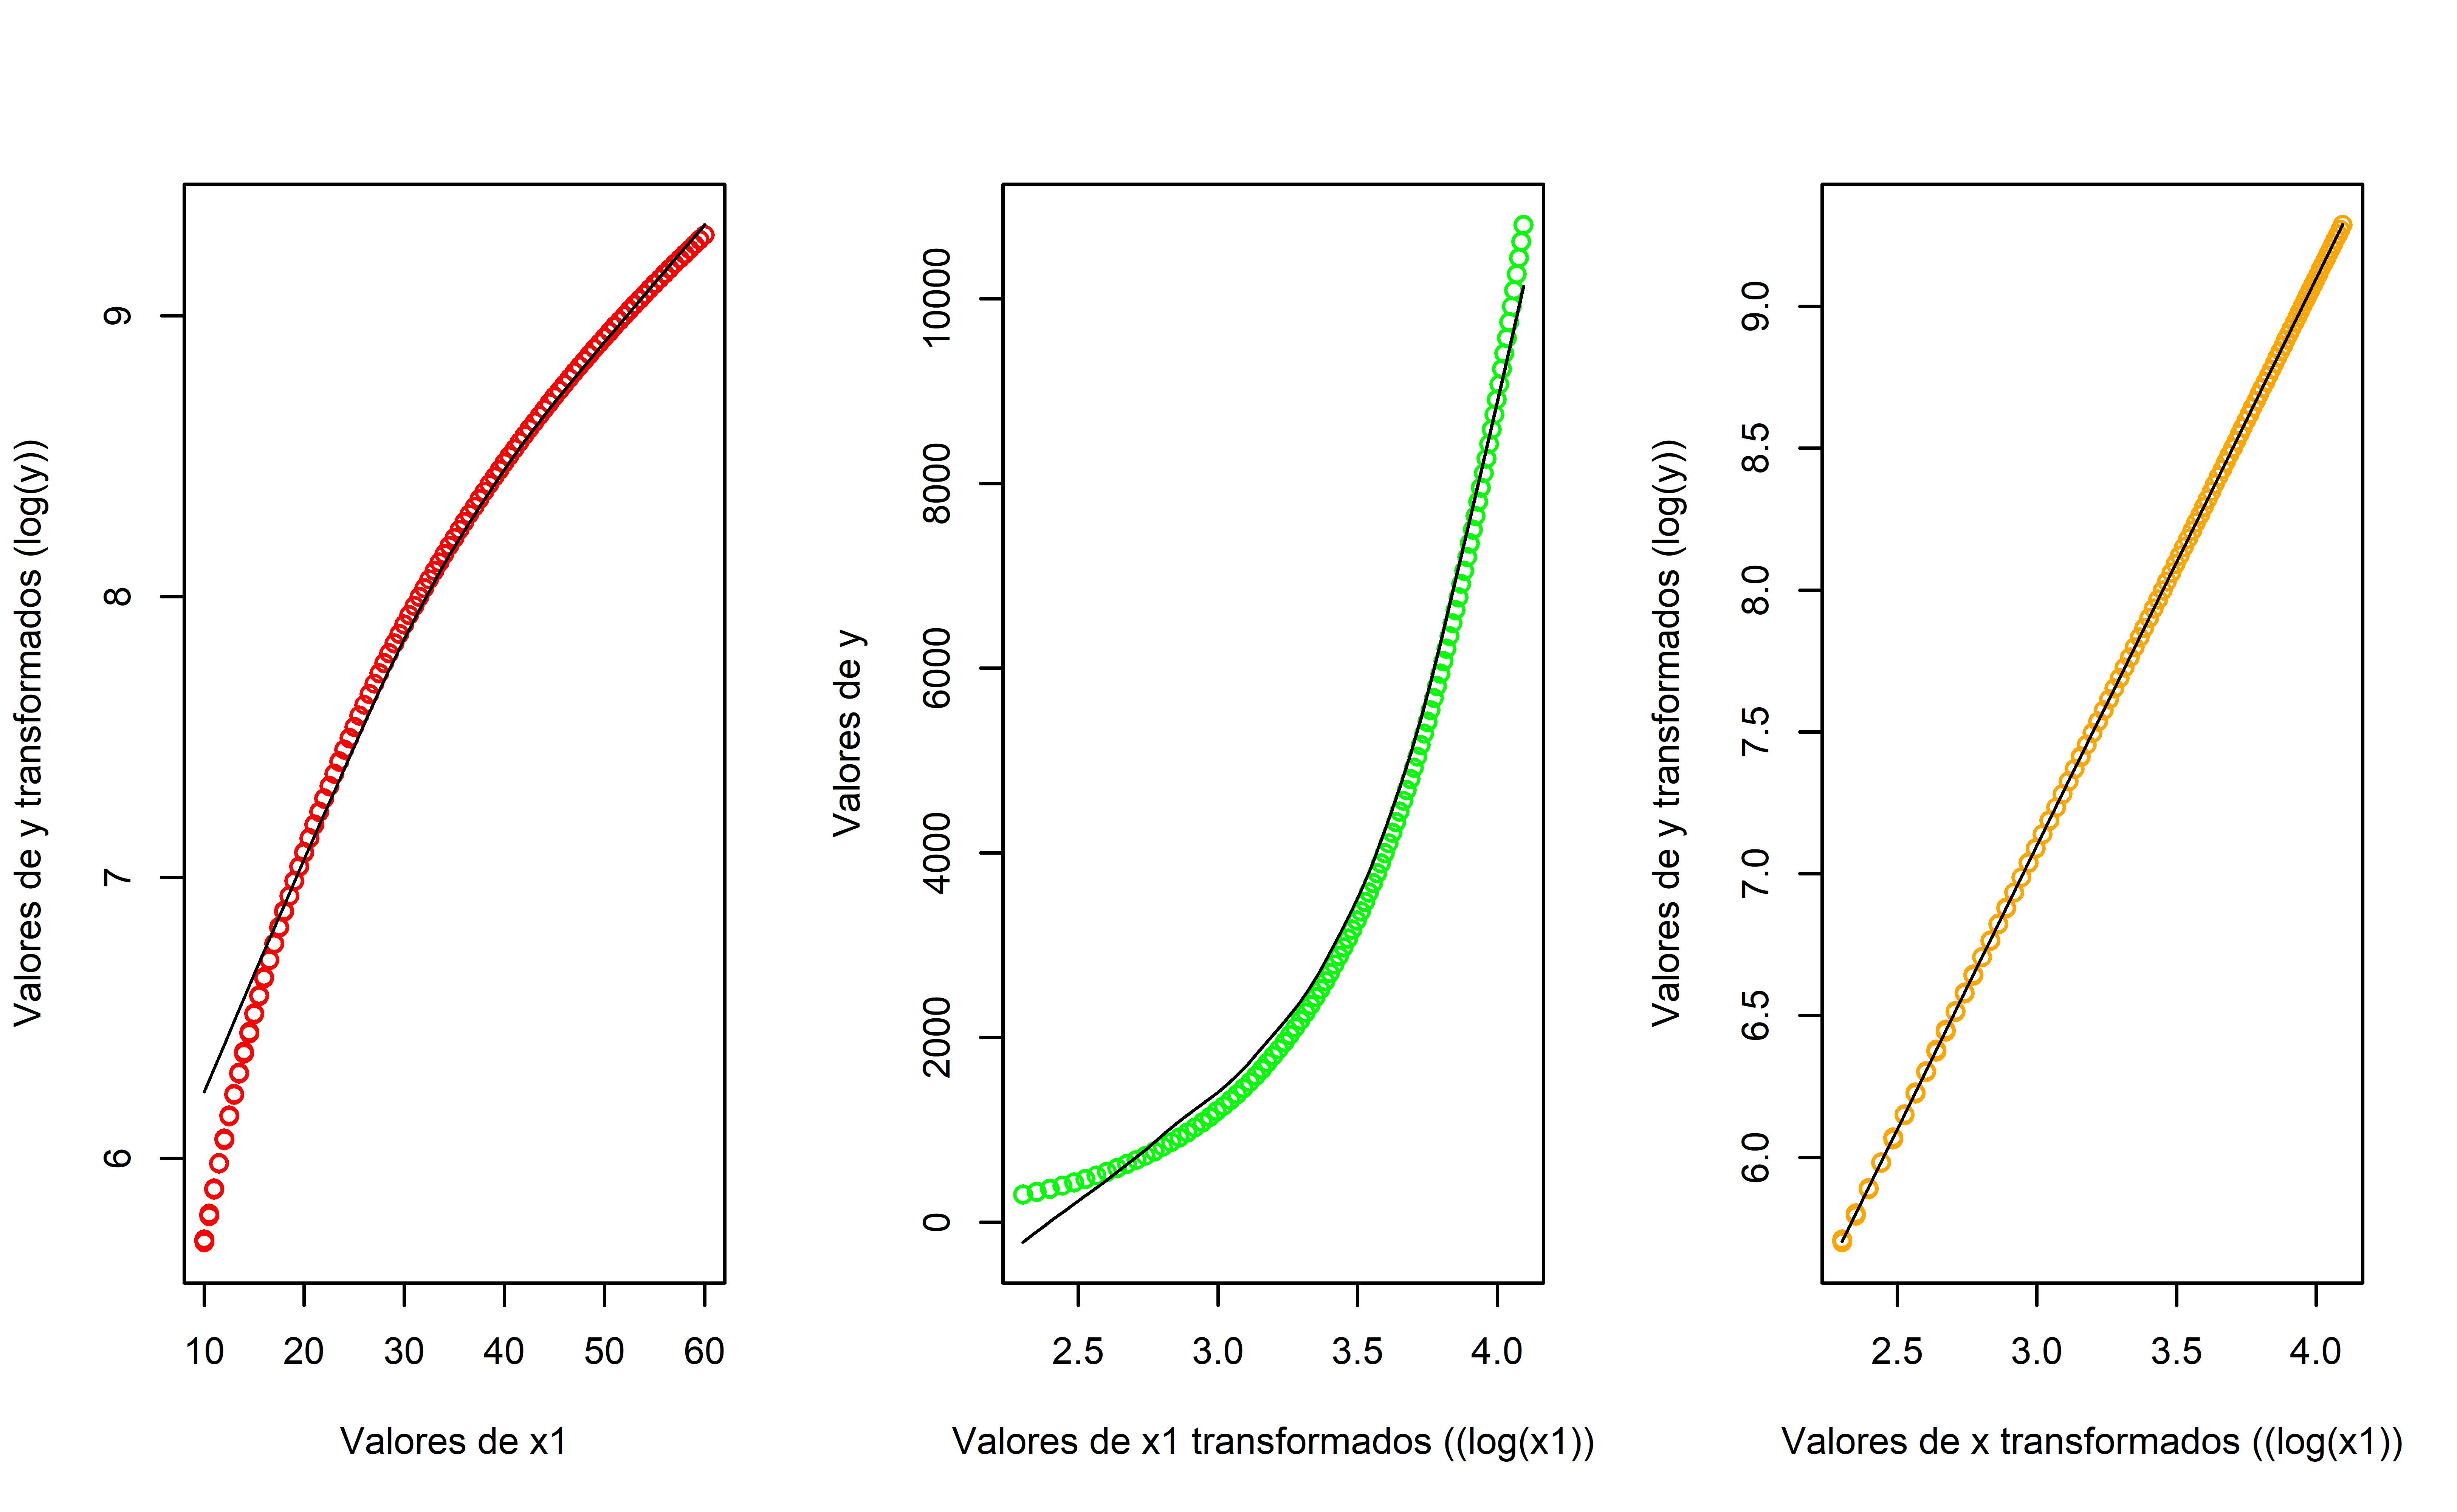
\includegraphics[scale=0.6]{Figures/graficaslog.png}
\caption{Comparativo de diagramas de dispersión con la transformación logarítmica}
\label{tlog}
\end{figure}

En la figura \ref{traiz}, se muestra el comparativo de los diagramas de dispersión de las transformaciones de raíz cuadrada aplicadas, tanto a los datos de las variables $x$, como a $y$ y a ambas, en la cual podemos observar que se obtiene un ajuste lineal a los datos cuando se aplica la transformación logarítmica a los datos de la variable, así mismo, su coeficiente de determinación $R^2 = 1$.

\begin{figure}
\centering
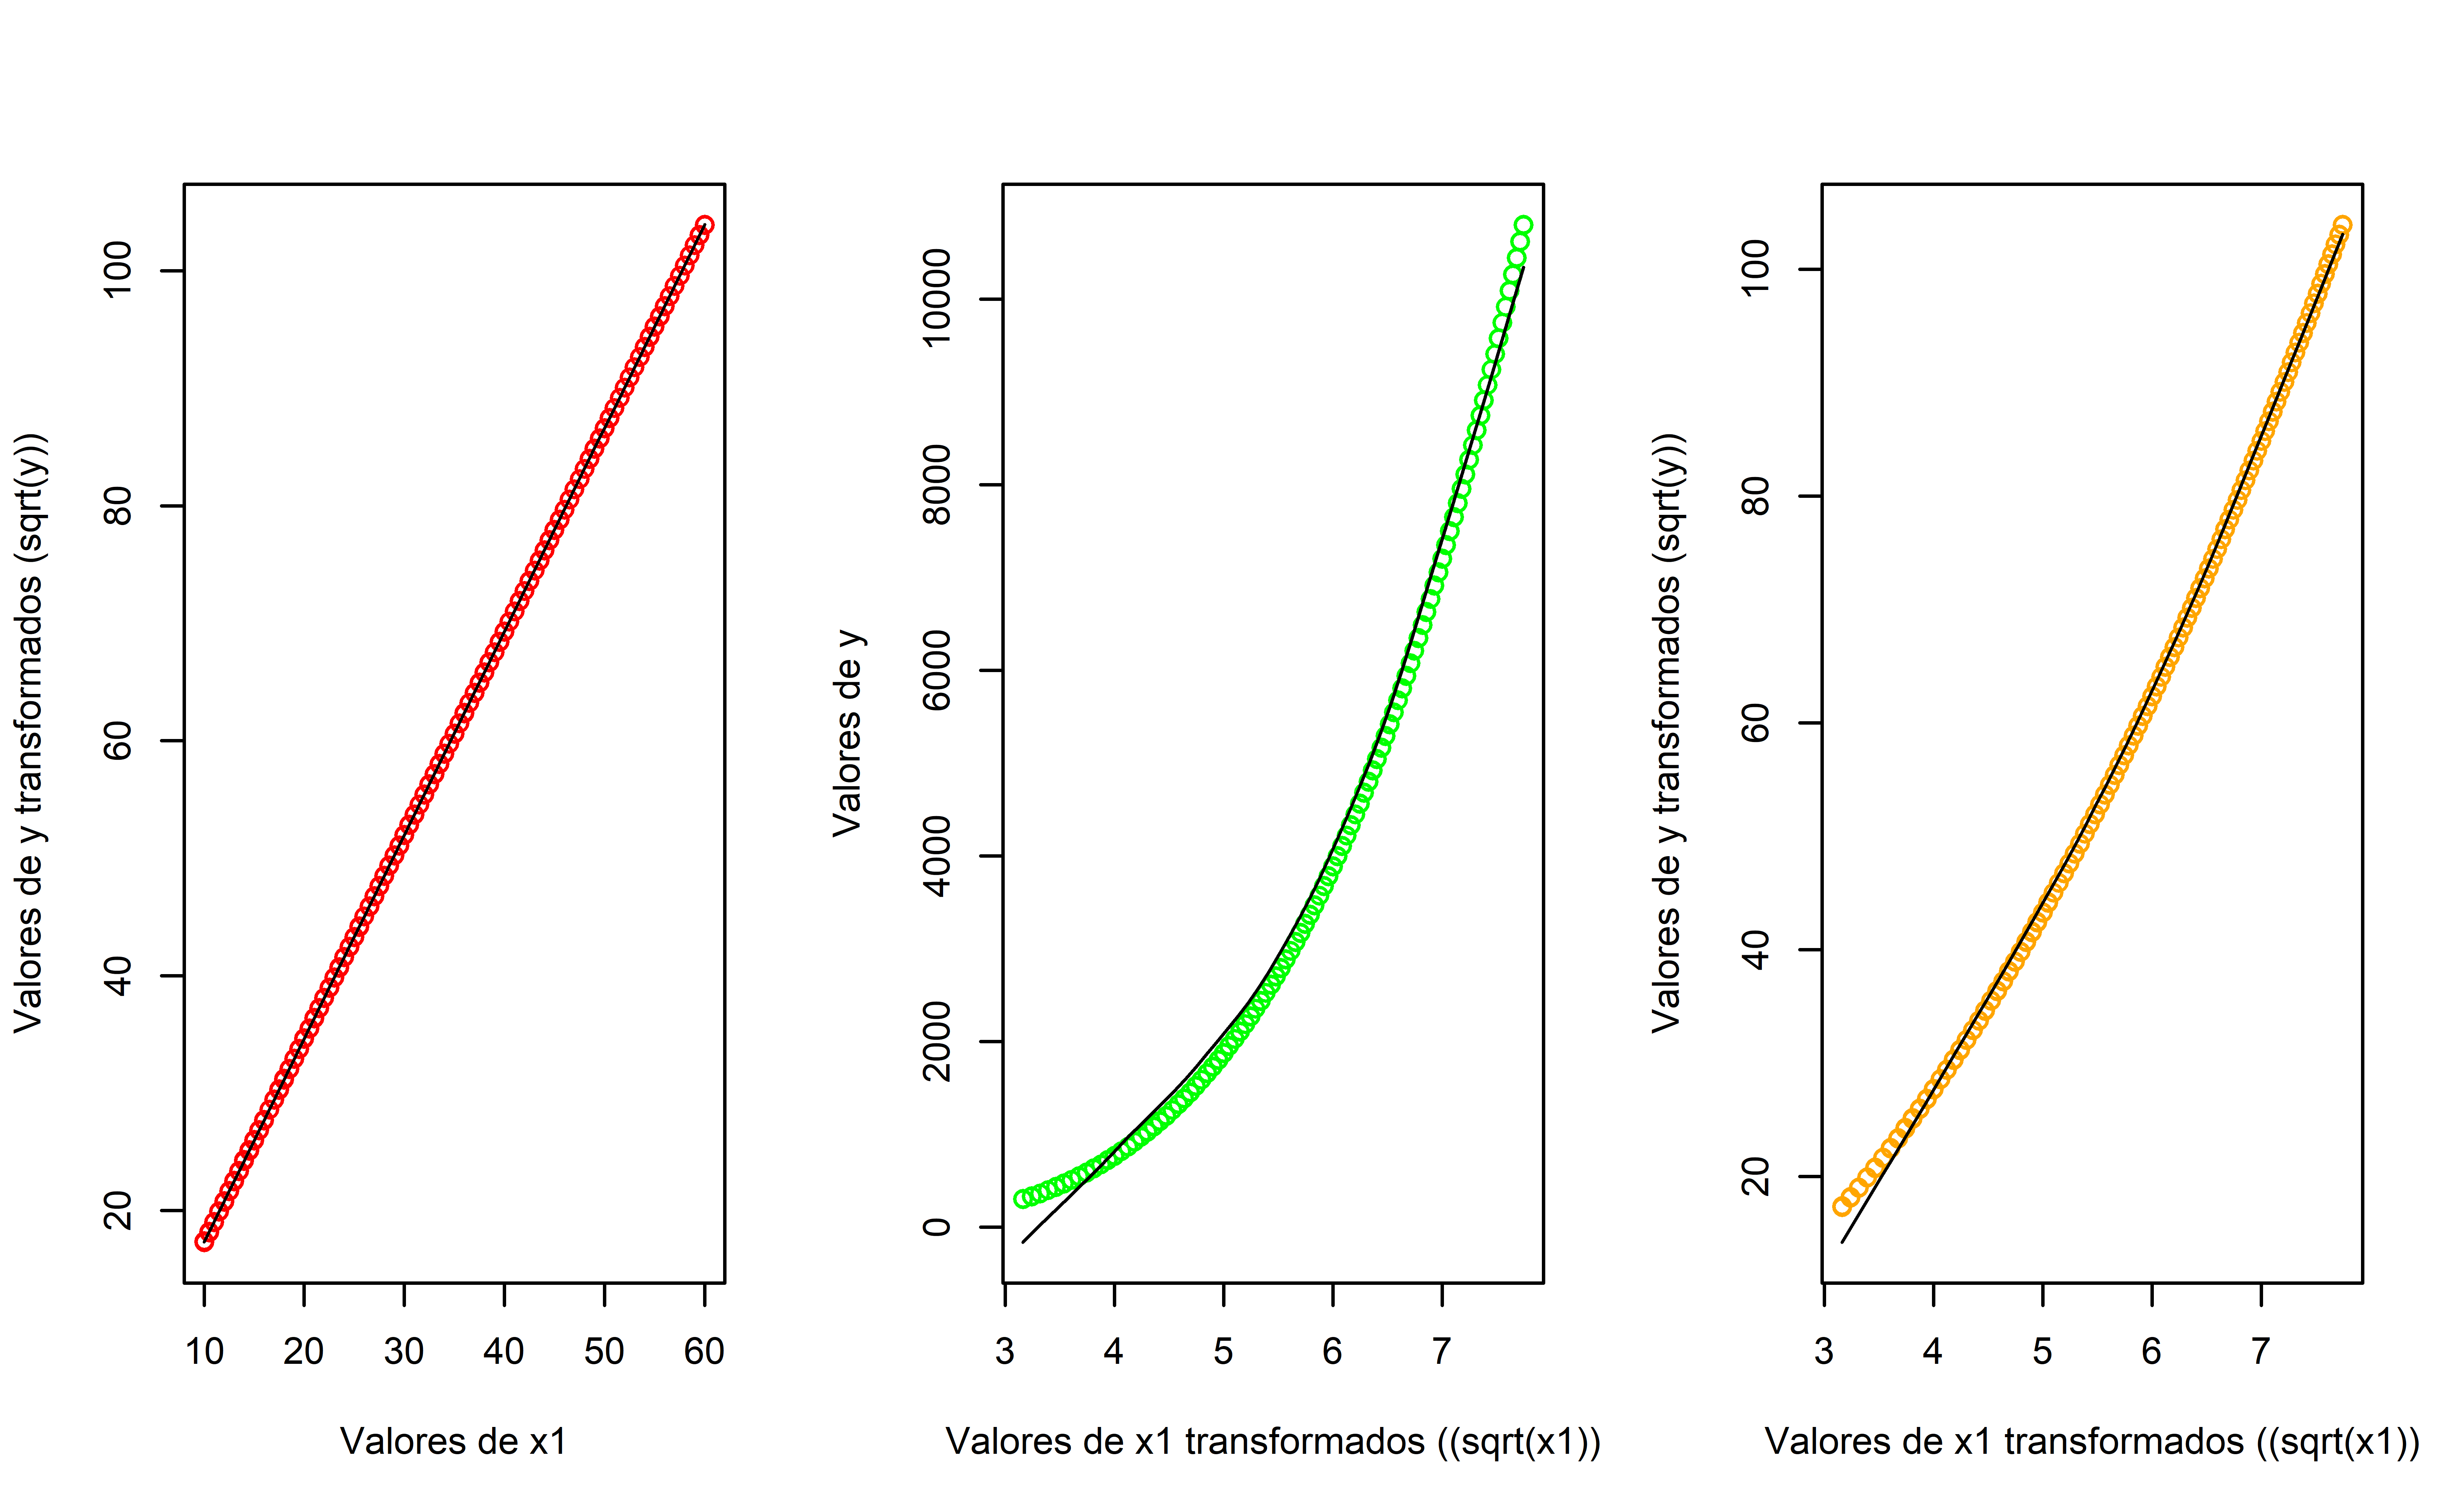
\includegraphics[scale=0.5]{Figures/graficasraiz.png}
\caption{Comparativo de diagramas de dispersión con la transformación de raíz cuadrada}
\label{traiz}
\end{figure}

Finalmente, en la figura \ref{tbox}, se muestra el diagrama de dispersión de la transformación Box\textendash Cox, en la cual se puede observar que al igual que con la transformación logarítmica de $x$ y $y$ o la raíz cuadrada de $y$, los datos se logran ajustar a relación lineal. Además, para estas trasformaciones el coeficiente de determinación fue $R^2 =1$. El valor de lambda para estos datos es de $\lambda = 0.505$.

\begin{figure}[h]
\centering
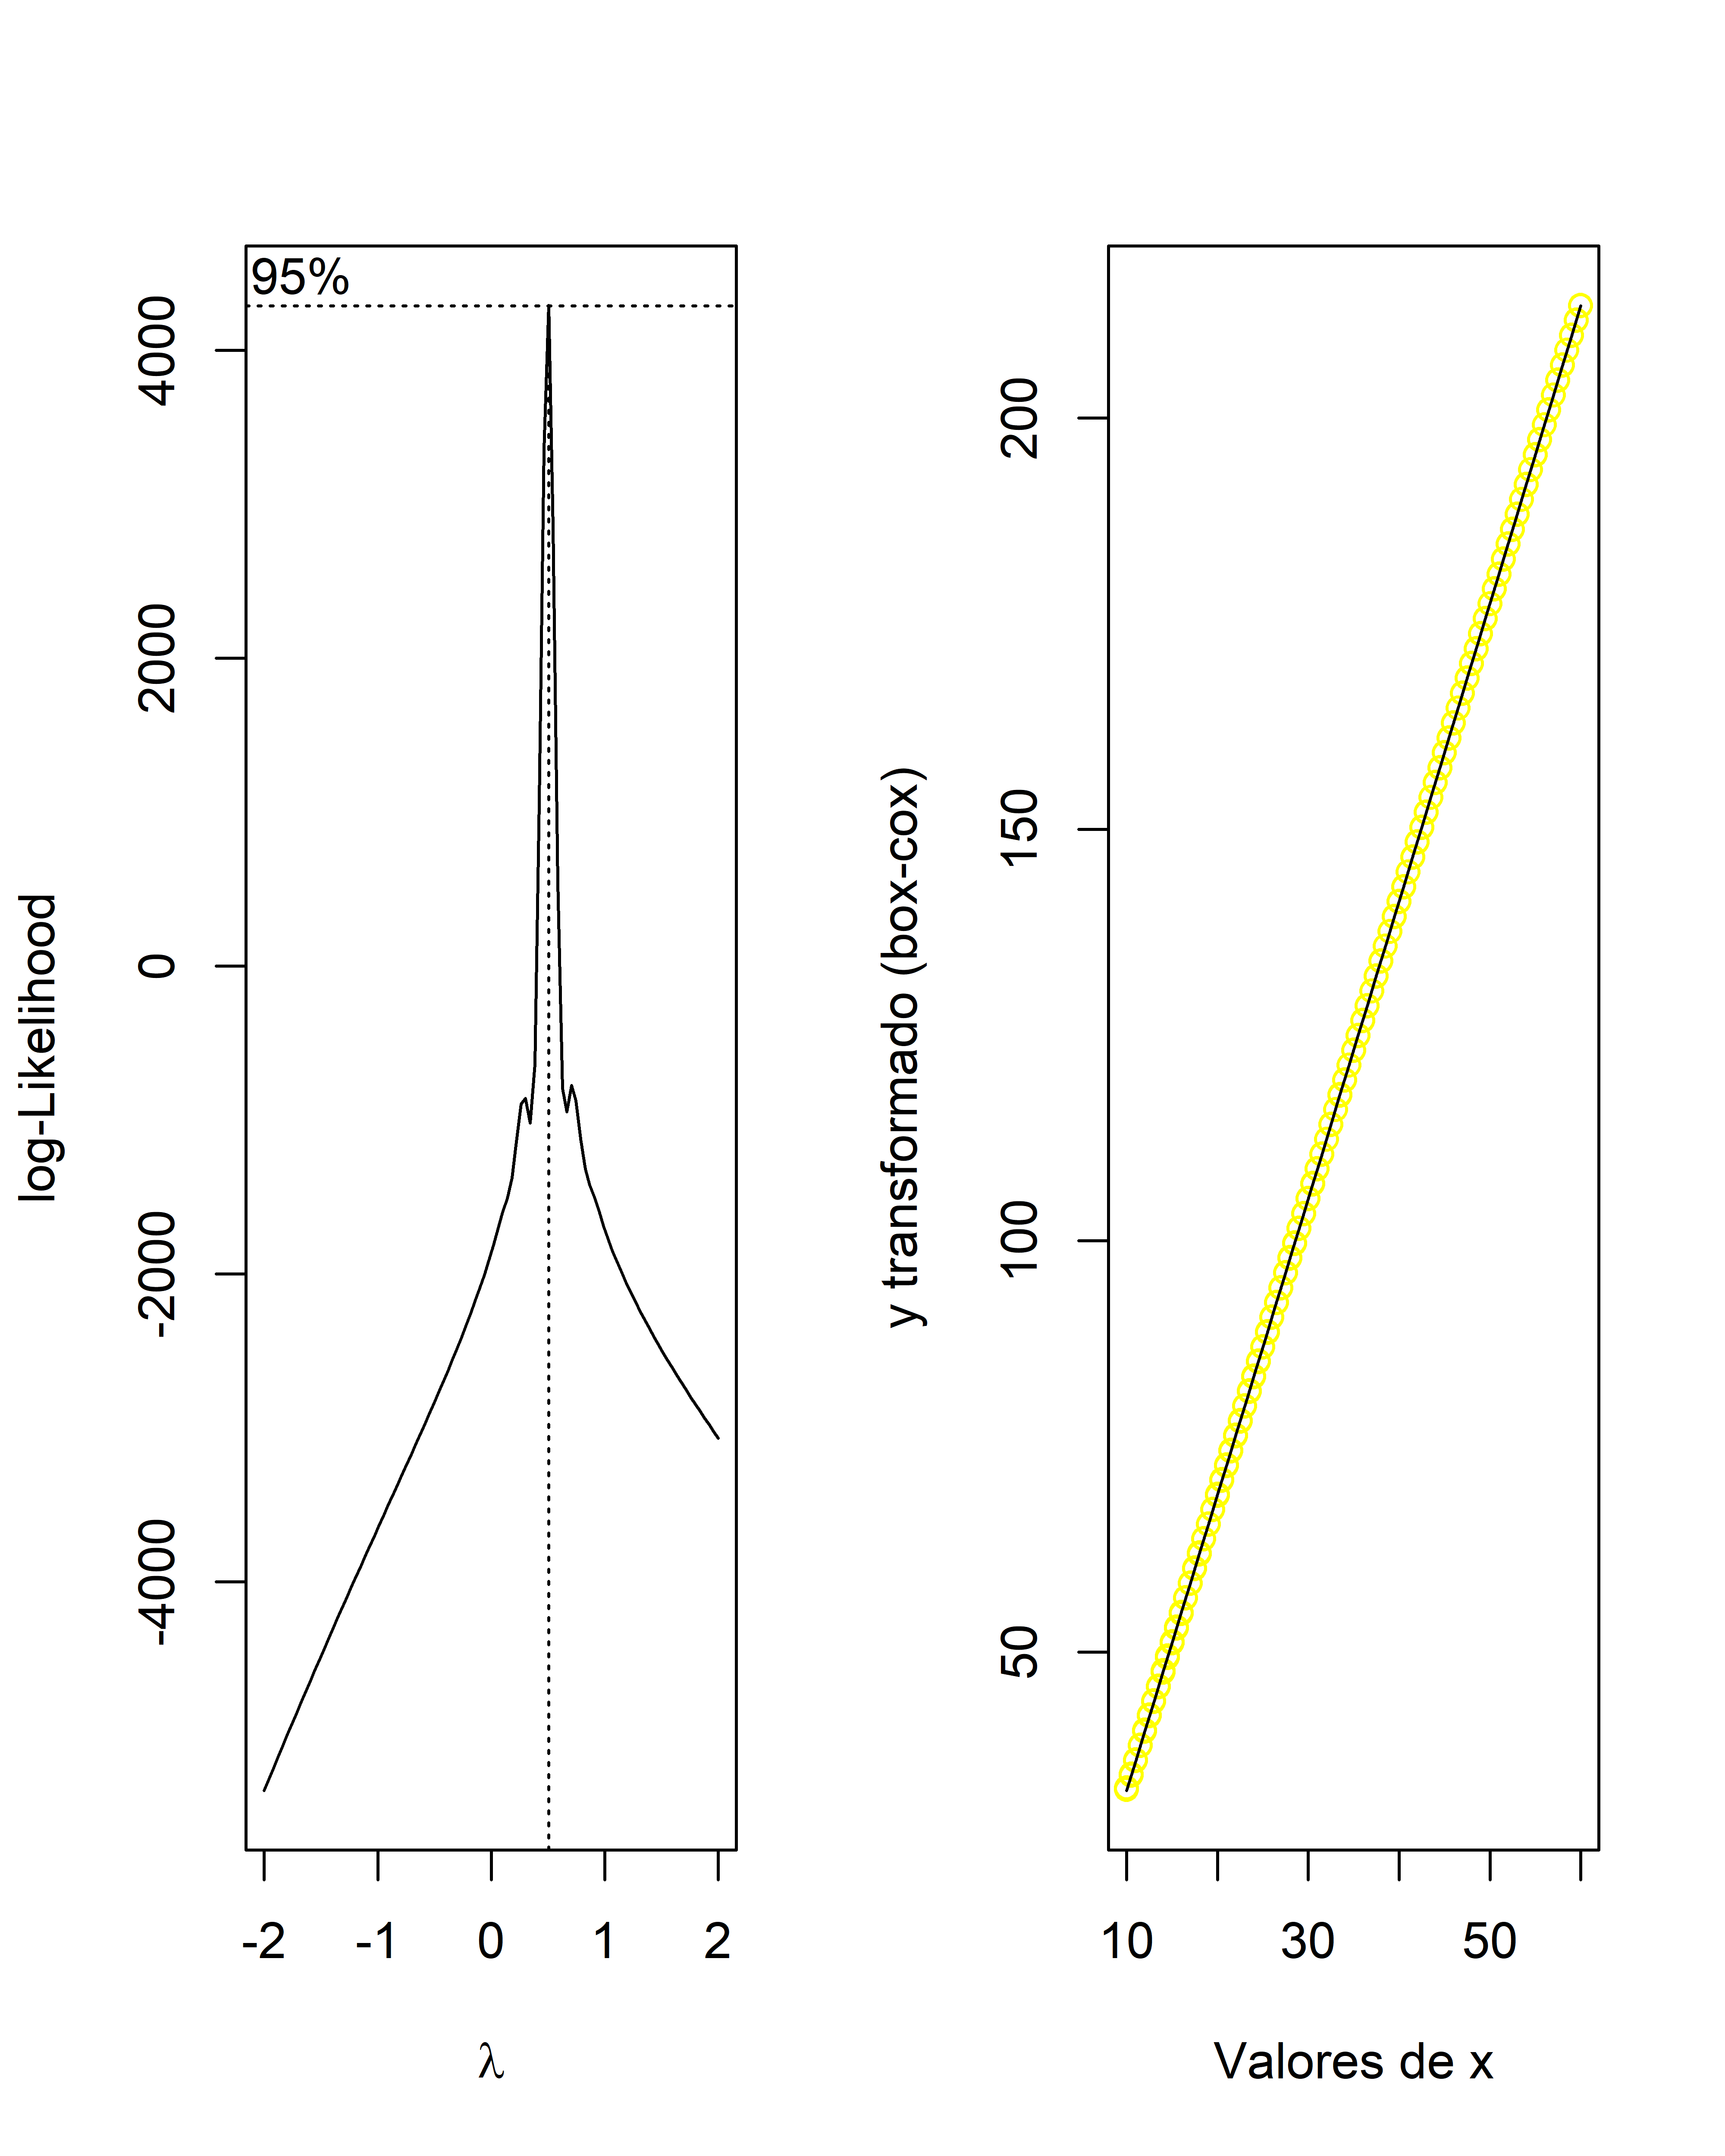
\includegraphics[scale=0.5]{Figures/graficabox.png}
\caption{Valores de lambda ($\lambda$) y diagrama de dispersión con la transformación de Box\textendash Cox}
\label{tbox}
\end{figure}

\VerbatimInput{Resulpruebas/boxcox.txt}

Para efectos prácticos, se consideraron los datos obtenidos de la aplicación de la función \texttt{lm} con la transformación de Box\textendash Cox (aunque también es válido escoger cualquiera de las tres buenas trasformaciones obtenidas), para determinar el modelo estimado de regresión lineal simple. De acuerdo a los resultados arrojados, se observa que $\hat{b}_{1} = 3.60$, $\hat{b}_{0} = -3.07$. Por lo tanto, el modelo estimado de regresión lineal simple para estos datos estaría dado como $\hat{y}=3.60x_{1}-3.07$. Adicionalmente, se realizó el mismo procedimiento considerando que los valores de la variable $x_{1}$ tuvieran otro tipo de distribución y para este caso, no se obtuvieron los mismos resultados, haciendo que las transformaciones propuestas no fueron suficientes. En el programa R, la rutina \texttt{assumptions(lm)} de la librería \textit{trafo}, permite obtener información acerca de varias transformaciones que cumplan con los supuestos de un modelo lineal de los datos que estamos analizando.

Para la regresión lineal múltiple, también se generaron $1,000$ datos a partir de la ecuación no lineal con dos variables independientes. Los resultados obtenidos fueron guardados en un dataframe. Se utilizo la función \texttt{cor} para determinar la correlación entre estas variables. Las respectivas correlaciones se encuentran graficadas en la figura \ref{multiple}, en la cual se puede observar que no hay una dependencia lineal de $y$ con las variables $x_{1}$ y $x_{2}$

\begin{figure}[h]
\centering
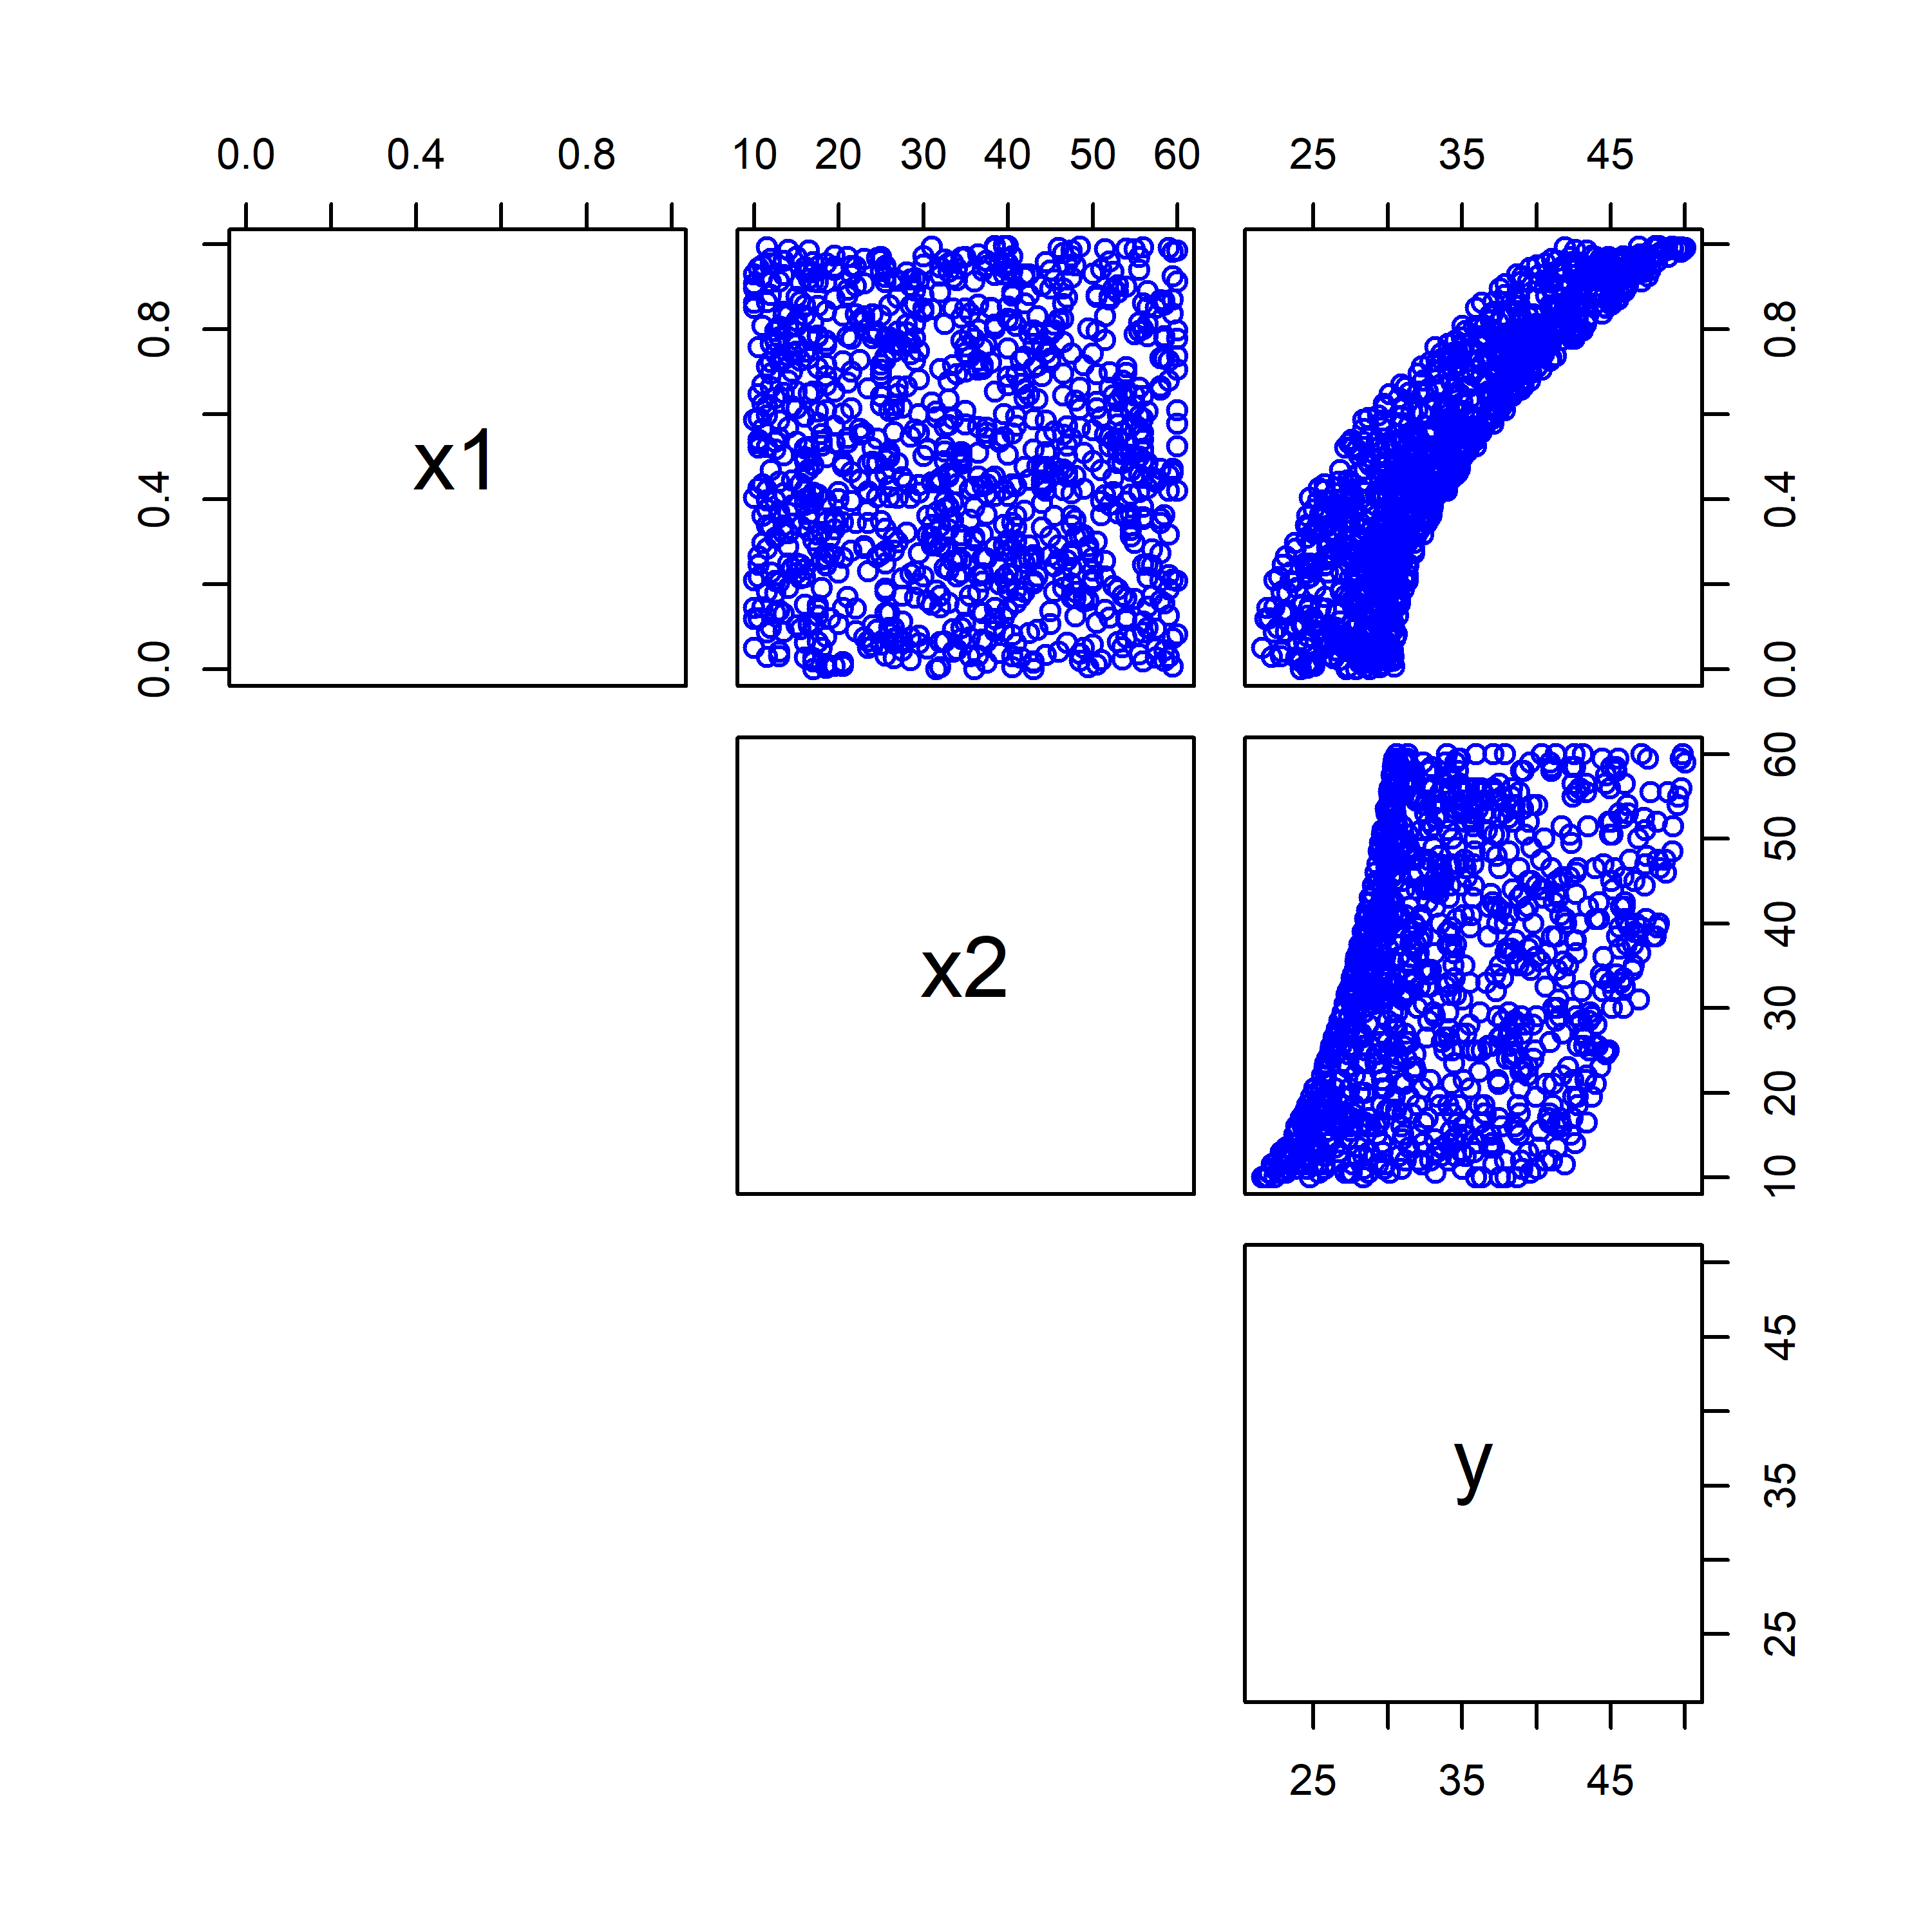
\includegraphics[scale=0.7]{Figures/multiplenolineal.png}
\caption{Correlación entre los datos provenientes de una ecuación no lineal con dos variables independientes}
\label{ec1}
\end{figure}

Se aplicaron las transformaciones logarítmicas, de raíz cuadrada y Box\textendash Cox, de las cuales, la transformación ($\log y$) presentó el mejor $R^2 =0.9519$, es decir, es capaz de explicar el $95.19\%$ de la variabilidad observada en los datos. De acuerdo a los resultados arrojados, se observa que $\hat{b}_{1} = 0.586$, $\hat{b}_{2} = 0.005$ y $\hat{b}_{0} = 3.035$. Por lo tanto, el modelo estimado de regresión lineal múltiple para estos datos estaría dado como $\hat{y}=0.586x_{1} + 0.005x_{2} + 3.035$, lo que significa que, si el resto de variables se mantienen constantes, por cada unidad que aumenta el predictor en cuestión, la variable $y$ varía en promedio tantas unidades como indica la pendiente. Para este ejemplo, por cada unidad que aumenta el predictor $x_{1}$, el valor de $y$ aumenta en promedio $0.586$ unidades, manteniéndose constante la variable $x_{2}$.

\VerbatimInput{Resulpruebas/multiplenolineal.txt}


\bibliography{refProbabilidad}
\bibliographystyle{plain}

\end{document}

El procedimiento Box\textendash Cox está incluido en el paquete MASS con la función boxcox . Utiliza un procedimiento de log-verosimilitud para encontrar la lambda que se utilizará para transformar la variable dependiente de un modelo lineal (como un ANOVA o una regresión lineal). También se puede utilizar en un solo vector.

Aquí, utilizo la función transformTukey , que realiza pruebas iterativas de Shapiro-Wilk y encuentra el valor lambda que maximiza la estadística W de esas pruebas. En esencia, esto encuentra la transformación de poder que hace que los datos se ajusten lo más posible a la distribución normal con este tipo de transformación.




La función transformTukey en el paquete rcompanion encuentra la lambda que hace que un solo vector de valores, es decir, una variable, se distribuya lo más normalmente posible con una simple transformación de potencia. 

 

El procedimiento Box – Cox está incluido en el paquete MASS con la función boxcox . Utiliza un procedimiento de log-verosimilitud para encontrar la lambda que se utilizará para transformar la variable dependiente de un modelo lineal (como un ANOVA o una regresión lineal). También se puede utilizar en un solo vector.

Debido a que log (0) no está definido, como lo es el logaritmo de cualquier número negativo, cuando se usa una transformación logarítmica, se debe agregar una constante a todos los valores para que todos sean positivos antes de la transformación. A veces, también es útil agregar una constante cuando se utilizan otras transformaciones.